%%
%% This is file `./samples/longsample.tex',
%% generated with the docstrip utility.
%%
%% The original source files were:
%%
%% apa7.dtx  (with options: `longsample')
%% ----------------------------------------------------------------------
%% 
%% apa7 - A LaTeX class for formatting documents in compliance with the
%% American Psychological Association's Publication Manual, 7th edition
%% 
%% Copyright (C) 2019 by Daniel A. Weiss <daniel.weiss.led at gmail.com>
%% 
%% This work may be distributed and/or modified under the
%% conditions of the LaTeX Project Public License (LPPL), either
%% version 1.3c of this license or (at your option) any later
%% version.  The latest version of this license is in the file:
%% 
%% http://www.latex-project.org/lppl.txt
%% 
%% Users may freely modify these files without permission, as long as the
%% copyright line and this statement are maintained intact.
%% 
%% This work is not endorsed by, affiliated with, or probably even known
%% by, the American Psychological Association.
%% 
%% ----------------------------------------------------------------------
%% 
\documentclass[man]{apa7}

\usepackage{lipsum}

\usepackage[american]{babel}

\usepackage{csquotes}
\usepackage[style=apa,sortcites=true,sorting=nyt,backend=biber]{biblatex}
\DeclareLanguageMapping{american}{american-apa}
\addbibresource{bibliography.bib}

% \title{Analyzing sensory judgments made by people and machines}

% \author{Alexander Ku}
% \affiliation{Department of Psychology, Princeton University}

% \leftheader{Ku}
% \title{Sample APA-Style Document Using the \textsf{apa7} Package}
% \shorttitle{Sample Document}

\title{Analyzing sensory judgments made by people and machines}
\shorttitle{PSY503 Final Paper}

\author{Alexander Ku}
\affiliation{Department of Psychology, Princeton University}

\leftheader{Ku}

\abstract{This report reproduces some of the statistical analysis performed by \cite{marjieh2023language}, which shows that sensory judgments from a large language model are highly predictive of human sensory judgments across multiple modalities. Furthermore, they also find no stronger correlation for visual judgments over non-visual judgments, despite the language model they use (GPT-4) being trained on both visual and linguistic data. Note that I've slightly modified the analysis as to better fit the content of this class.}

\keywords{APA style, statistics, reproduction, similarity, perception}


\authornote{
   % \addORCIDlink{Daniel A. Weiss}{0000-0000-0000-0000}

  Correspondence concerning this article should be addressed to Alexander Ku, Department of Psychology, Princeton University, Peretsman Scully Hall, Princeton, NJ 08540.  E-mail: alexku@princeton.edu}

\begin{document}
\maketitle

\section{Method}

We begin with a concise exposition of the hypothesis and data collection procedure. A thorough methodological description can be found in the original paper. The objective of this section is parsimony: to provide minimally sufficient information to understand the statistical analysis being performed.

\subsection{Hypotheses}

A key question of interest to cognitive scientists and philosophers alike is the extent to which linguistic description can express and convey sensory experience. The authors posit a philosophical thought experiment: can an alien anthropologist (oxymoron?) infer the idiosyncrasies of an alien species' perceptual experience from the language they speak? For example, a species that can see infrared may have words to describe colors that are indistinguishable to people. In the setting we are interested in, the large language model is the anthropologist, and we are the alien species.

Thus, the hypothesis we will be testing is as follows: are large language models predictive of human sensory experience? Concretely, are perceptual similarity judgments from a large language model, solicited via linguistic description, correlated with human similarity judgments, solicited via sensory stimuli.

\cite{marjieh2023language} test this hypothesis for both visual and non-visual stimuli. They find that the similarity judgments from a large language model are significantly and strongly correlated with human similarity judgments. Furthermore, they show that, despite the large language model they use (GPT-4) being trained on both visual an linguistic data, there is no significant difference between the correlation in similarity judgments for visual and non-visual stimuli.

In order to test these hypotheses the authors must have aligned human and model data. That is, human and model similarity judgments for the same stimulus pair. The authors use both preexisting data as well as collect their own using an online crowd-sourcing platform (Amazon Mechanical Turk).

\subsection{Collecting human data}

The authors consider 6 sensory dimension (color, loudness, timbre, taste, pitch, and vocal consonants) across 3 sensory modalities (visual, auditory, gustatory). Human similarity judgments for color, loudness, timbre, taste are pubicly available from previous studies. These data were collected using both online crowd-sourcing platforms as well as in the lab. The authors also collected additional similarity judgments for pitch and vocal consonants via online crowd-sourcing platform. Their detailed methodology can be found in the original manuscript.

These data contain pairwise similarity judgments for $n$ stimuli (per sensory dimension). This yields an $n\times n$ similarity matrix. Because similarity is a subjective measure, each entry in the matrix is averaged over 5 subjects. Entries of this matrix are normalized such that similarity is between 0 (`completely dissimilar') and 1 (`completely similar'). See Figure \ref{fig:sim_matrix} for a visualization.

\subsection{Collecting machine data}

To collect aligned similarity judgments from a large language model (GPT-4), the authors must translate the sensory stimuli used by the human data into linguistic form. For example, color can be encoded as a hexadecimal code. Similarity judgments are solicited using in-context learning. Here is an example of a prompt the model sees for color:

\begin{verbatim}
People described pairs of colors using their hex
codes. How similar are the two colors in each
pair on a scale of 0-1 where 0 is completely
dissimilar and 1 is completely similar? Respond
only with the numerical similarity rating.
Color 1: #ff5700 Color 2: #ff9b00 Rating 0.76
Color 1: #b3ff00 Color 2: #00ff61 Rating: 0.45
Color 1: #FF0000 Color 2: #00b2ff Rating: 0.02
Color 1: <hex-code1> Color 2: <hex-code2>
Rating:
\end{verbatim}

As with people, model similarity judgments for each stimulus pair are collected multiple times. This is because large language models are stochastic---they decode text using a method called temperature sampling. The temperature indicates how much variability you have in your decoded samples. In theory, you can make decoding deterministic by setting the temperature to 0 or some epsilon value (i.e., greedy decoding), however this often degrades the quality of the samples. Thus, the authors decide to use the default temperature parameter and solicit 10 similarity judgments per stimulus pair, and average them to construct the similarity matrices. See Figure \ref{fig:sim_matrix} for a visualization.

\begin{figure}
    \centering
    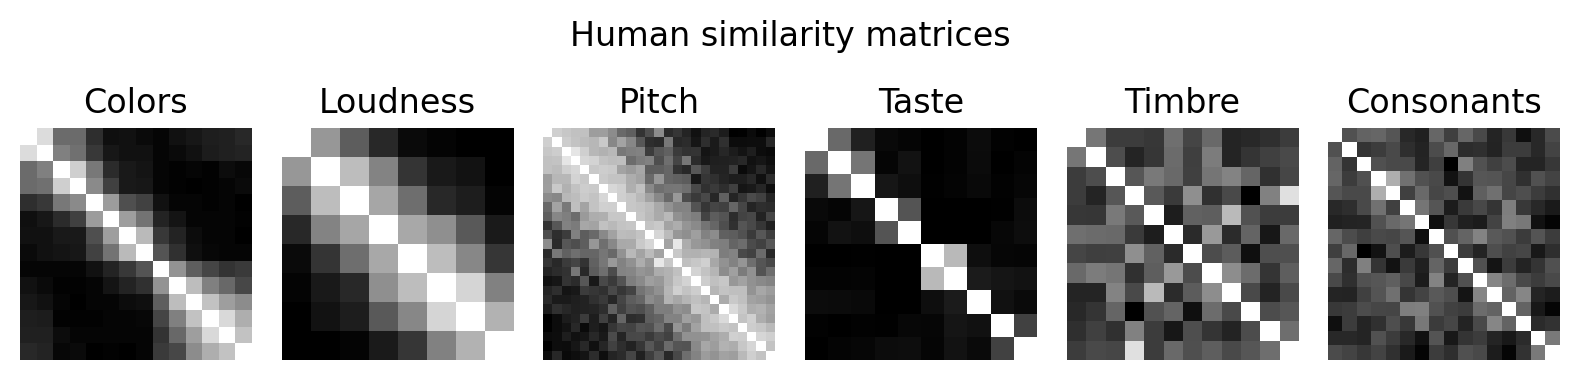
\includegraphics[width=\textwidth]{figures/human_sim.png}
    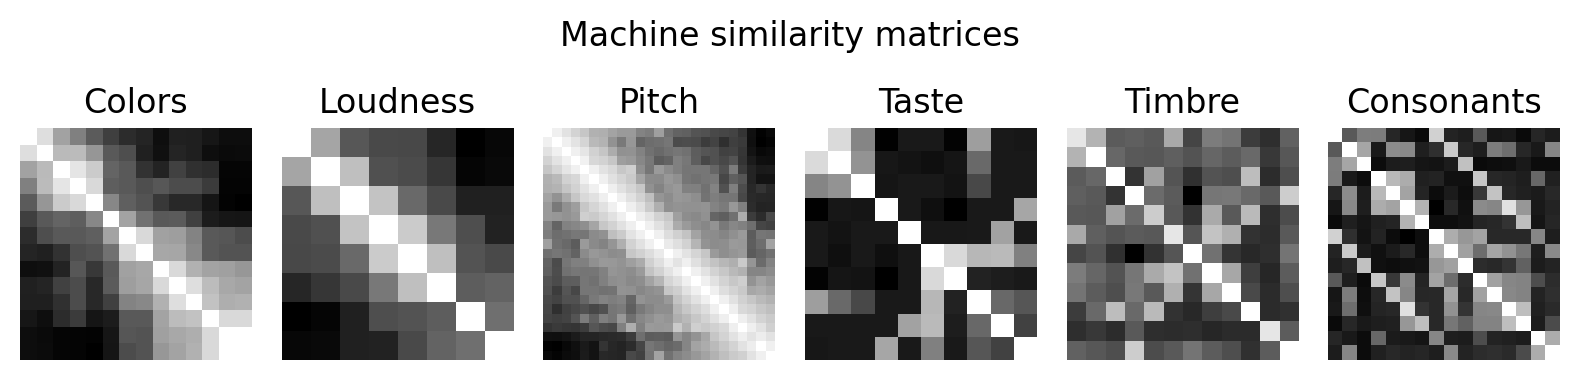
\includegraphics[width=\textwidth]{figures/mach_sim.png}
    \caption{Human and machine similarity matrices for each sensory dimension. Light pixels indicate high similarity, dark pixels indicate low similarity.}
    \label{fig:sim_matrix}
\end{figure}


\section{Do machine judgments predict human judgments?}

Now that we understand the type of data we are working with (i.e., pairwise similarity judgments across sensory dimensions), we will shift our focus to the first of the author's questions: do machine judgments predict human judgments?

Before we begin with the analysis, I will describe some preprocessing we do to the data. While similarity need not be commutative (as Tversky famously showed), for the stimuli we use, it is. Thus the resulting similarity matrices are also symmetric. For this reason, we will deduplicate (a.k.a., dedupe) our data. That is, when computing statistical measures, such as correlation, we will only use the upper triangular entries of the similarity matrix. Doing so leaves us with a dataframe containing 650 rows. Each row contains the index of the stimulus pair, the human similarity judgment for that pair, the machine similarity judgment for that pair, and the sensory dimension.

First, let's visualize the data using a scatter plot. As we can see in Figure \ref{fig:jointplot} there seems to be a relationship between human similarity and machine similarity. Running a correlation test tells us that there is a significant and strong positive correlation between the two variables, r = 0.79, 95\% CI [0.76, 0.82], t(64) = 33.08, p < .001. That is to say, when human similarity increase so does machine similarity, and vice versa.

\begin{figure}
    \centering
    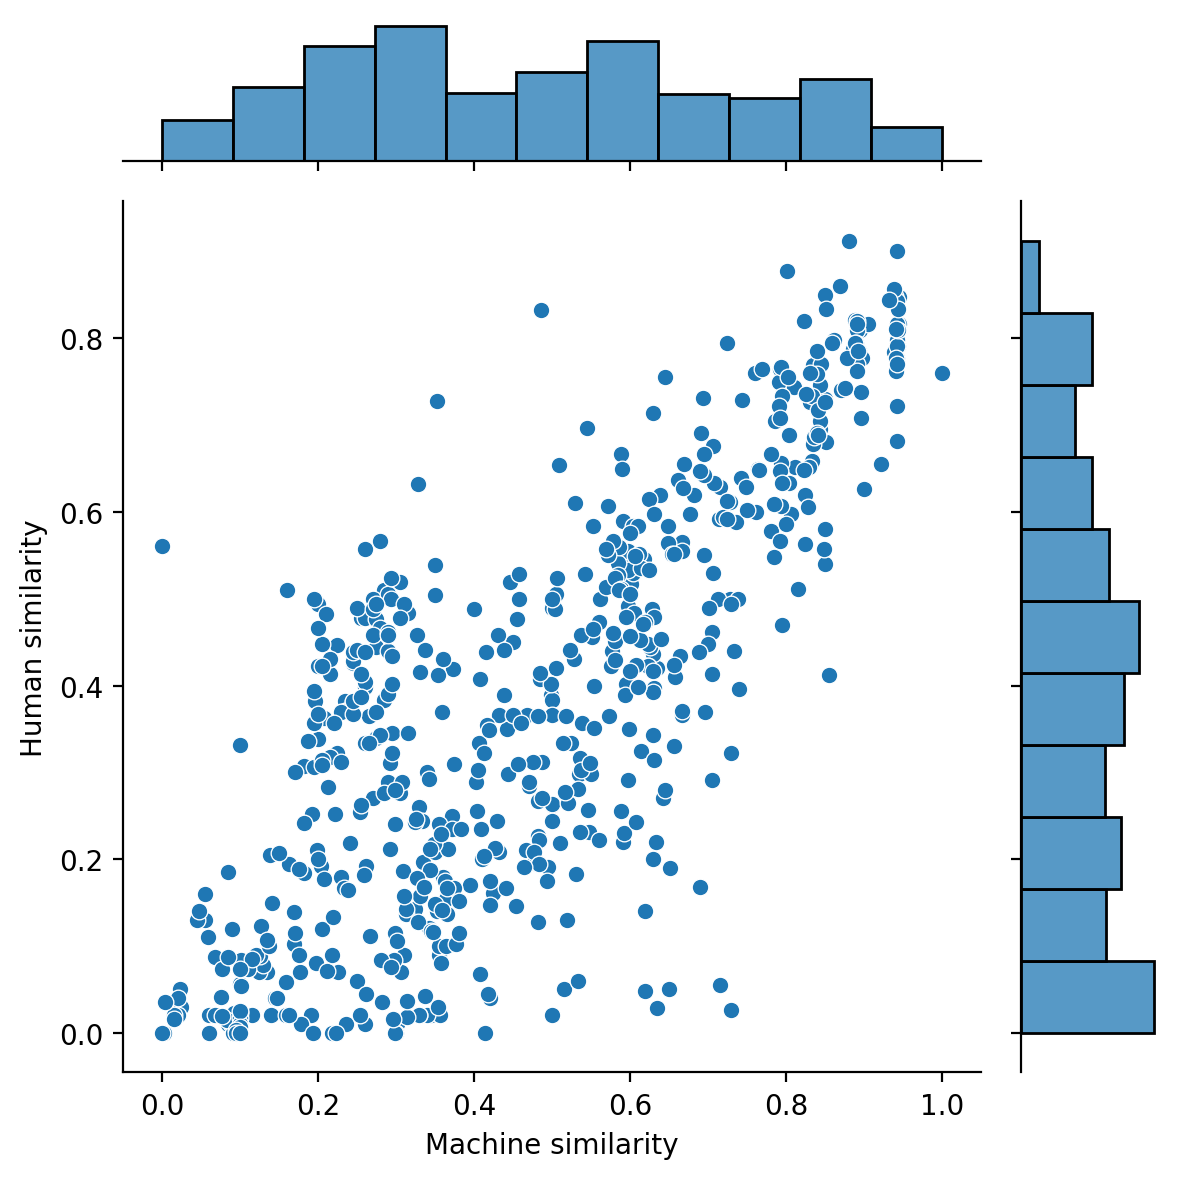
\includegraphics[width=\textwidth]{figures/jointplot.png}
    \caption{Scatter plot of human similarity judgments against machine similarity judgments. Marginal densities are visualized on the top and right as histograms.}
    \label{fig:jointplot}
\end{figure}

Now that we have established that the two variables are correlated, let's fit a linear regression. We will let machine similarity be the independent variable and human similarity be the dependent variable---that is we want to see if machine similarity is predictive of human similarity. The slope of the regression line is 0.759. This means that for every unit increase in machine similarity, there is a 0.759 increase in human similarity. However, because similarity is bounded between 0 and 1, this interpretation does not make sense. It makes more sense to say: for every 0.1 increase in machine similarity, human similarity increases by 0.0759. The intercept of the regression line is 0.0203. This means that when machine similarity is 0, the mean human similarity is 0.0203. The model explains a large and significant portion of the variation in the data (R2 = 0.628, F(1, 64) = 1095., p < .001, adj. R2 = 0.628). F-test tells us that it is significantly better than the empty model. The $R^2$ value tells us that 62.7\% of the variance in human similarity is explained by model similarity. The adjusted $R^2$ is the same as the regular $R^2$, since we only have one predictor. Figure \ref{fig:regplot} plots the regression line with 95\% confidence intervals. Figure \ref{fig:assumptions} tells us residuals of this model are normally distributed and homoskedastic.\footnote{The residuals are slightly misbehaved around 0 and 1 (i.e., where similarity saturates). Thus, it may be worth using a transformation (e.g., logit, probit), however, when I tried, the residuals were even more misbehaved. For now, we will proceed assuming the linear model is appropriate.}

\begin{figure}
    \centering
    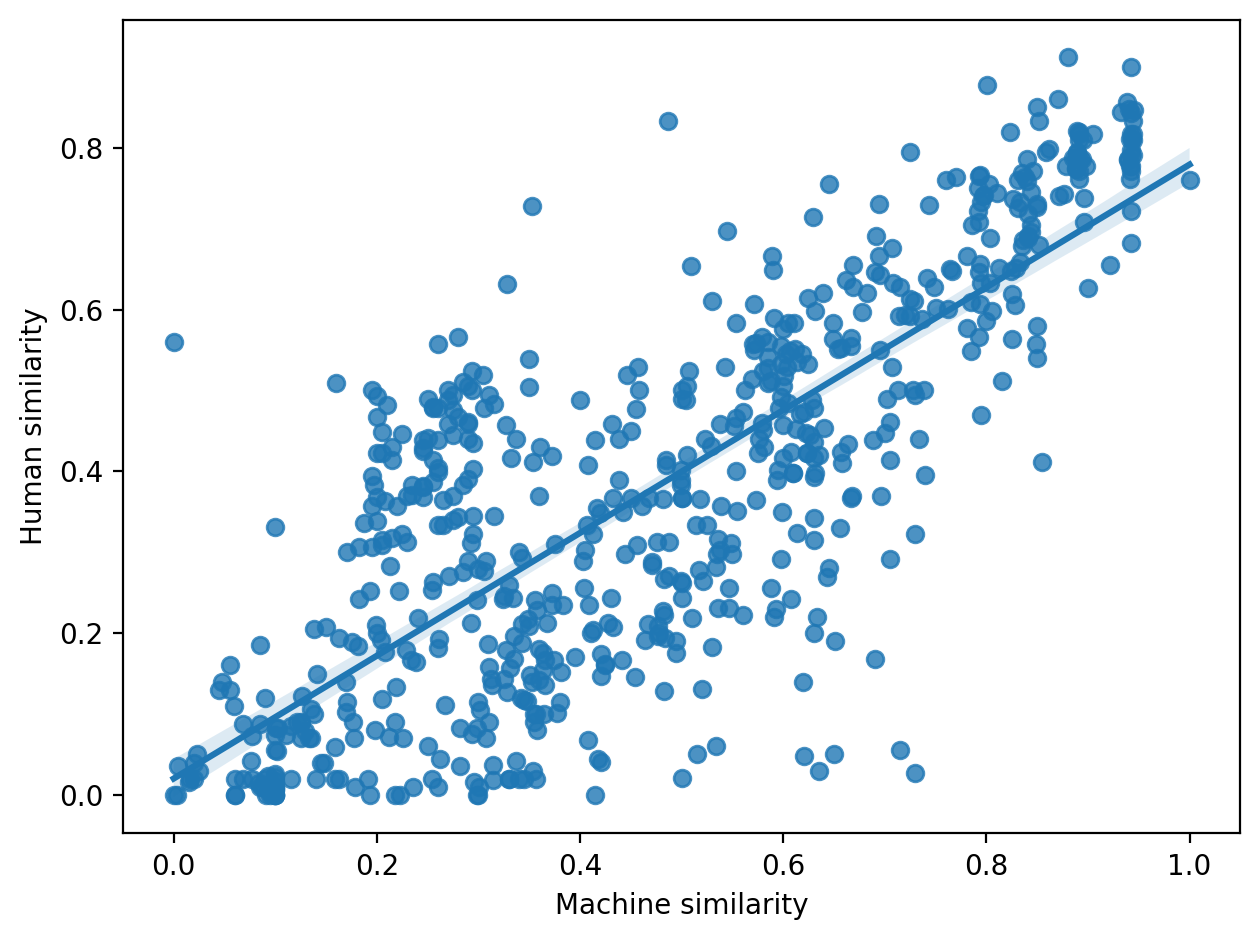
\includegraphics[width=\textwidth]{figures/regplot.png}
    \caption{Linear regression line with 95\% confidence intervals.}
    \label{fig:regplot}
\end{figure}

\begin{figure}
    \centering
    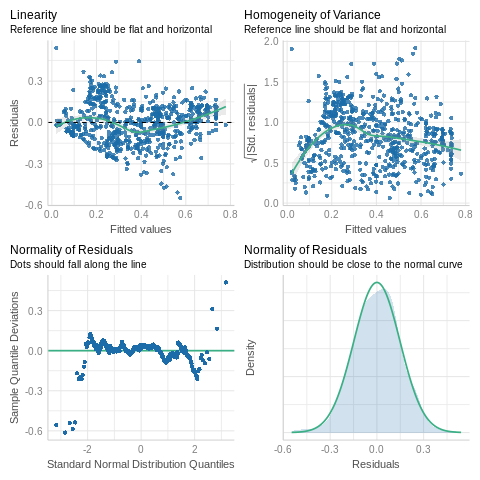
\includegraphics[width=\textwidth]{figures/assumptions.png}
    \caption{Residual checks for linear regression.}
    \label{fig:assumptions}
\end{figure}

% \begin{verbatim}
% We fitted a linear model (estimated using OLS) to predict human_data with
% machine_data (formula: human_data ~ machine_data). The model explains a
% statistically significant and substantial proportion of variance (R2 = 0.63,
% F(1, 648) = 1094.50, p < .001, adj. R2 = 0.63). The model's intercept,
% corresponding to machine_data = 0, is at 0.02 (95% CI [-4.03e-03, 0.04], t(648)
% = 1.64, p = 0.102). Within this model:

%   - The effect of machine data is statistically significant and positive (beta =
% 0.76, 95% CI [0.71, 0.80], t(648) = 33.08, p < .001; Std. beta = 0.79, 95% CI
% [0.75, 0.84])

% Standardized parameters were obtained by fitting the model on a standardized
% version of the dataset. 95% Confidence Intervals (CIs) and p-values were
% computed using a Wald t-distribution approximation.
% \end{verbatim}

\section{Does the effect differ between visual and non-visual stimuli?}

The large language model the authors use (GPT-4) is trained on both visual an linguistic data, yet they find there is no significant difference in the relationship between human similarity and machine similarity for visual and non-visual stimuli. Let's perform a moderation analysis to determine whether visual vs. non-visual is a moderator. To facilitate this analysis we add a factor to our dataframe indicating whether the similarity is being measured for visual or non-visual stimuli. First, we will plot regression lines to visualize the interaction. As we can see in in Figure \ref{fig:regplot2} there does not seem to be an interaction.

\begin{figure}
    \centering
    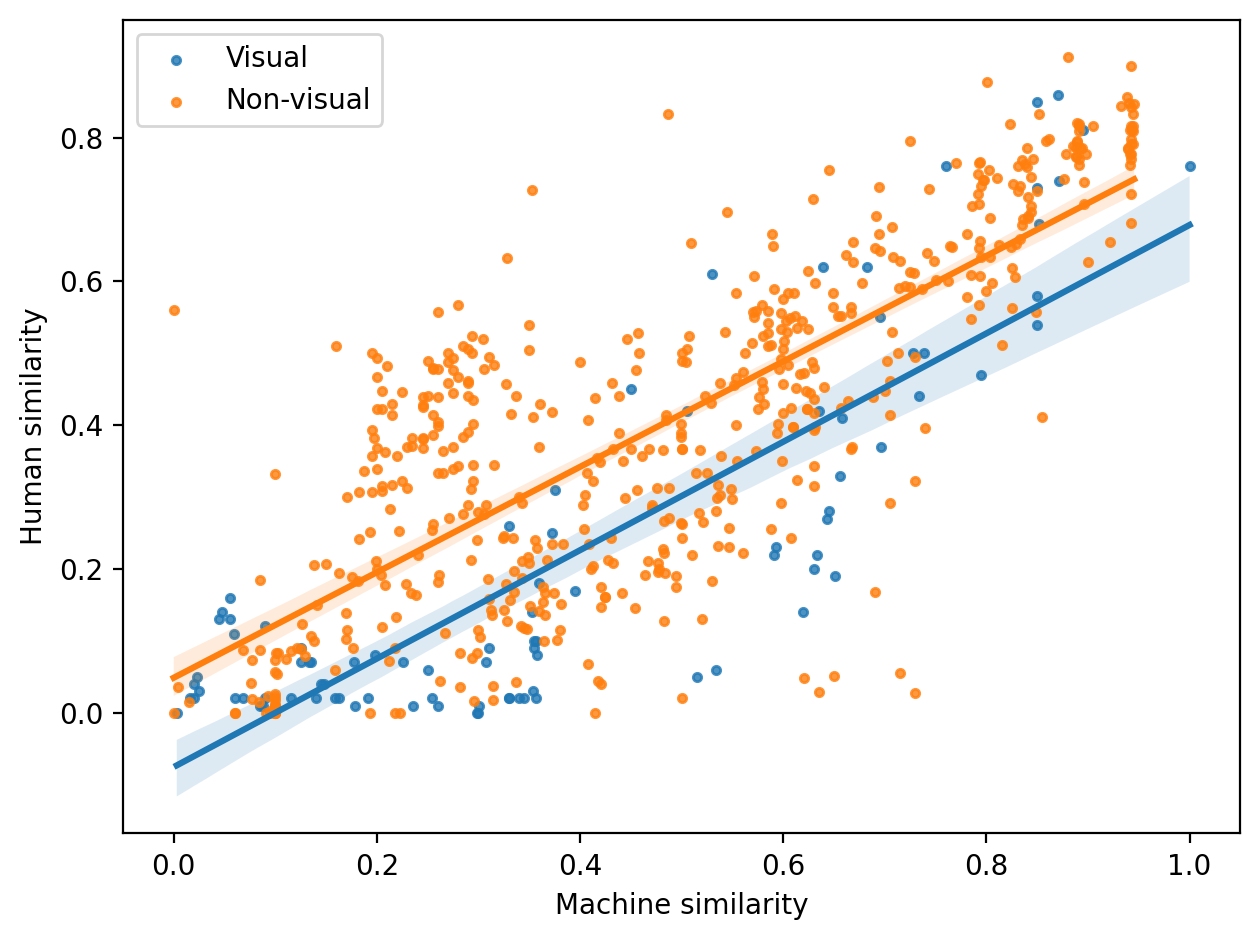
\includegraphics[width=\textwidth]{figures/regplot2.png}
    \caption{Linear regression lines for similarities of visual and non-visual stimuli.}
    \label{fig:regplot2}
\end{figure}

Let's fit a multiple regression model where the dependent variable is human similarity and the independent variables are mean centered machine similarity, dummy coded visual factor, and an interaction term (i.e., product of machine similarity and visual factor). This results in a model that explains a statistically significant and substantial proportion of variance (R2 = 0.65, F(3, 646) = 408.60, p < .001, adj. R2 = 0.65).

The model's intercept is 0.40 (95\% CI [0.39, 0.41], t(646) = 65.34, p < .001) and indicates the predicted human similarity when machine similarity is at its mean and the stimuli are non-visual. The effect of machine similarity is statistically significant and positive (beta = 0.73, 95\% CI [0.69, 0.78], t(646) = 29.98, p < .001; Std. beta = 0.77, 95\% CI [0.72, 0.81]); every 0.1 increase in machine similarity results in a 0.073 increase in human similarity when the stimuli are non-visual. The effect of the visual factor is statistically significant and negative (beta = -0.11, 95\% CI [-0.15, -0.08], t(646) = -6.75, p < .001; Std. beta = -0.16, 95\% CI [-0.21, -0.12]); the intercept is 0.11 lower (i.e., the predicted change in human similarity) for visual stimuli when machine similarity is at its mean---this offset can be seen in Figure \ref{fig:regplot2}. Finally, the interaction effect is not statistically significant whatsoever (beta = 0.02, 95\% CI [-0.10, 0.14], t(646) = 0.34, p = 0.733; Std. beta = 7.45e-03, 95\% CI [-0.04, 0.05]); consistent with what the authors report. Finally, we'll calculate power. The smallest effect size we can observe with 99\% power is 0.02---which means we can observe small effects given the sample size ($n=650$).

\section{Discussion}

To summarize, our analysis is consistent with claims of the authors: (1) machine similarity judgments are highly predictive of human similarity judgments; and (2) whether the similarity is measured for visual or non-visual stimuli does not change this interaction, despite the model being trained on visual data.

Finally, I would like to end with a discussion of future directions this line research may pursue; as it is related to my own interests.

As cognitive psychologists, we infer mental processes and representations from behavior, often assuming that the behavior people exhibit is the (resource-)rational solution to a computational task. If the behavioral pattern of people and machines are aligned, and consistent with a mathematical theory (e.g., Bayesianism, connectionism), it is evidence that both systems have learned a similar solution and or internal representation. 

Rather than inferring representations from behavior, cognitive neuroscientists look inside the system itself. While brain imaging techniques (e.g., fMRI, EEG) have spatial or temporal resolution constraints, observing the numerical processing that happens inside of a large language model (a deep neural network) does not.

Many theories in cognitive psychology posit that stimuli are represented as points in a psychological metric space (e.g., Euclidean, hyperbolic). By studying the internal activations of a large language model, we can explicitly assess the embedding geometry of each layer of the network. And, like cognitive neuroscientists, we can develop mechanistic theories of perceptual semanticity that are consistent with behavioral ones, without the resolutional limitations of brain imaging.

\printbibliography

\end{document}

%% 
%% Copyright (C) 2019 by Daniel A. Weiss <daniel.weiss.led at gmail.com>
%% 
%% This work may be distributed and/or modified under the
%% conditions of the LaTeX Project Public License (LPPL), either
%% version 1.3c of this license or (at your option) any later
%% version.  The latest version of this license is in the file:
%% 
%% http://www.latex-project.org/lppl.txt
%% 
%% Users may freely modify these files without permission, as long as the
%% copyright line and this statement are maintained intact.
%% 
%% This work is not endorsed by, affiliated with, or probably even known
%% by, the American Psychological Association.
%% 
%% This work is "maintained" (as per LPPL maintenance status) by
%% Daniel A. Weiss.
%% 
%% This work consists of the file  apa7.dtx
%% and the derived files           apa7.ins,
%%                                 apa7.cls,
%%                                 apa7.pdf,
%%                                 README,
%%                                 APA7american.txt,
%%                                 APA7british.txt,
%%                                 APA7dutch.txt,
%%                                 APA7english.txt,
%%                                 APA7german.txt,
%%                                 APA7ngerman.txt,
%%                                 APA7greek.txt,
%%                                 APA7czech.txt,
%%                                 APA7turkish.txt,
%%                                 APA7endfloat.cfg,
%%                                 Figure1.pdf,
%%                                 shortsample.tex,
%%                                 longsample.tex, and
%%                                 bibliography.bib.
%% 
%%
%% End of file `./samples/longsample.tex'.
